\documentclass[../main.tex]{subfiles}

\begin{document}

\subsection{Uncertainty Estimation}
\label{sec:uncertainty}

\begin{figure}[H]
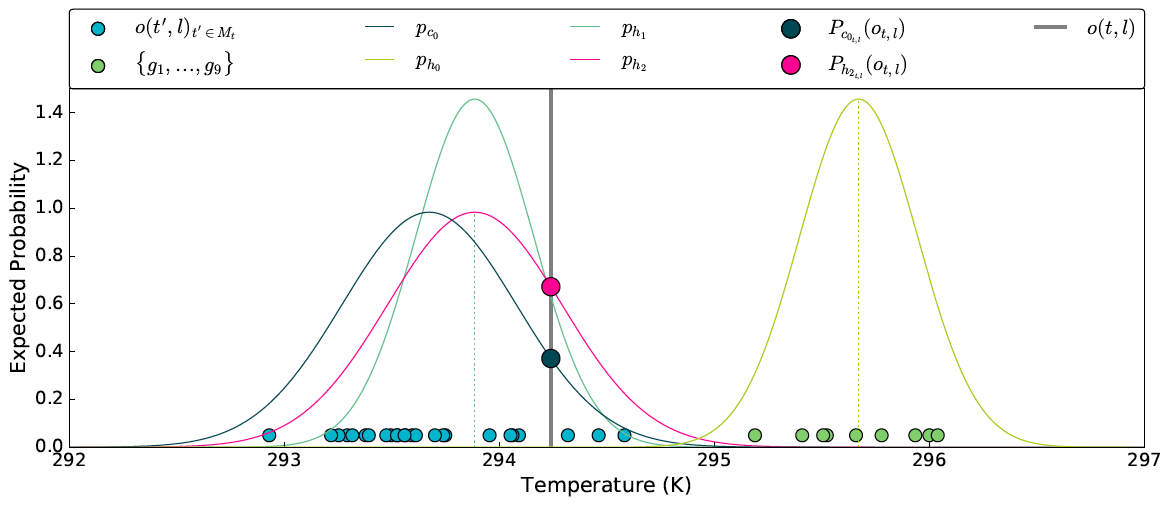
\includegraphics[width=1\textwidth]{uncertainty.png}
\caption{A model based on previous observations (light blue) and a model based on bias-corrected forecasts (pink) underestimated the likelihood of the temperature being around 294.15 at a grid point in the equatorial Atlantic ocean. The standard deviation of the model curves can be used as a proxy for how certain the models are about their predictions; the narrower observation model was more certain than the bias-corrected forecast model.\cite{aizenman_ensemble_2016}}
\label{fig:uncertainty}
\end{figure}

Another way to explore the probability distribution of semantically complex datasets is to leverage the field of uncertainty visualizations. As data analysis becomes increasingly probabilistic, there is a need to visualize the certainty of a model's prediction. As seen in figure~\ref{fig:uncertainty}, a model based on previous observations (light blue) and one based on a bias-corrected forecast (pink)) expected the temperature to be lower then it actually was\cite{aizenman_ensemble_2016}. The narrower standard deviation of the model based on observations indicates that the observation model was more confident of its prediction than the bias-corrected forecast model. A visualization of this uncertainty would try to show the deviation or a comparable measure of uncertainty. The measuring and encoding of uncertainty suggests methods for represent the structure of functional probabilistic distributions in a discrete less structurally complex manner. 

\subsubsection{Bivariate Choropleth}
\begin{figure}[H]
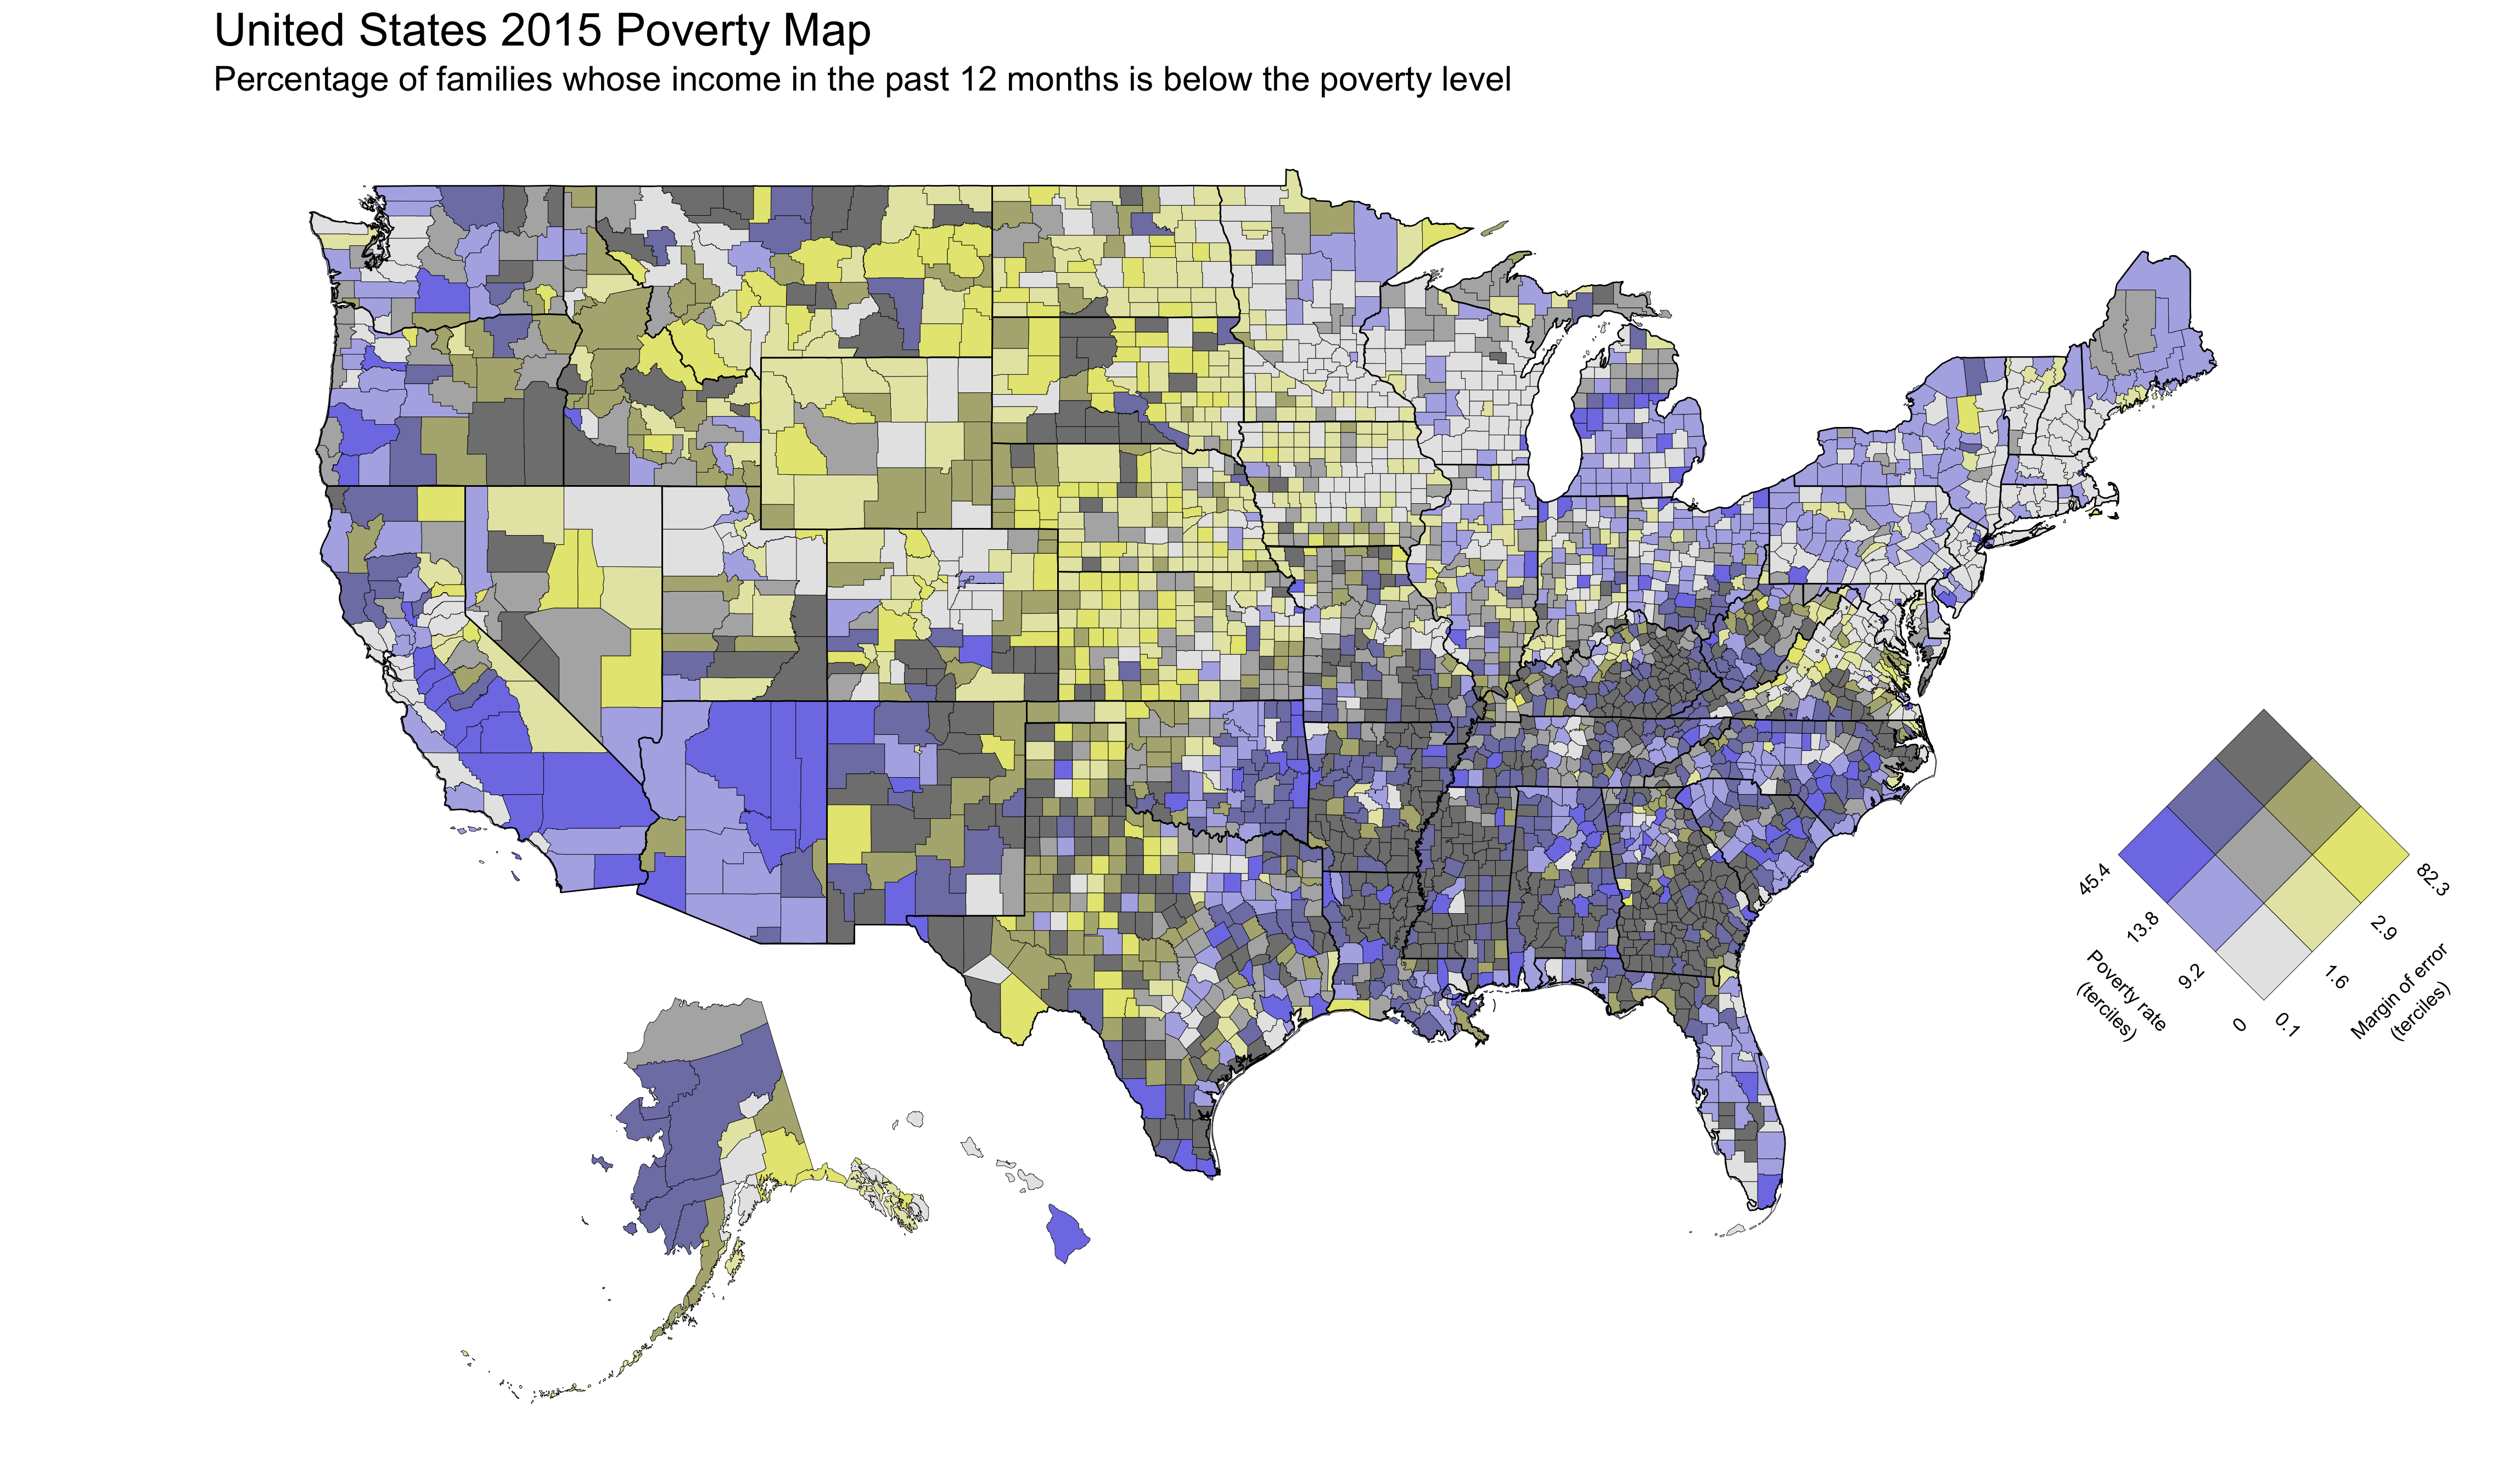
\includegraphics[width=1\textwidth]{bivariate.png}
\caption{American Community Survey poverty rates are encoded using shades of blue and the margin of error is in shades of yellow. Regions that are dark gray have a high poverty rate, but the measurement has a high margin of error. Figure is from \textit{Visualizing uncertainty in areal data} \cite{lucchesi_visualizing_2017}}
\label{fig:bivariate}
\end{figure}
One of the difficulties of visualizing data on maps is that the map takes up the x and y axis, so it is no longer available for other variables. In figure~\ref{fig:bivariate}, bivariate colormaps \cite{trumbo_theory_1981,carstensen_hypothesis_1986} are used to encode the poverty rate and margin of error in each American Community Survey tract. The advantage of using the bivariate colormap is that the uncertainty of the data is encoded in the same symbol as the data itself. This technique easily translates to representing a probability distribution of values at a location as a mean and standard deviation. The bivariate colormap can also natively be used to show conditional dependencies when the events are dependent on location. In figure~\ref{fig:bivariate}, the high poverty and low response rates across the southeastern cotton belt are reminiscent of many other socioeconomic patterns common to that region. The biggest limit of bivariate colormaps is that they can be difficult to read \cite{carstensen_hypothesis_1986}.


A full survey of uncertainty visualization techniques is outside the scope of this paper, but many such methods are listed in \textit{Visualization and Visual Analysis of Multifaceted Scientific Data: A Survey} \cite{kehrer_visualization_2013} and \textit{Visualizing High-Dimensional Data: Advances in the Past Decade} \cite{liu_visualizing_2017}.

\end{document}